\documentclass{article}

\usepackage{tikz}
\usepackage[inner=0.5cm,outer=0.5cm]{geometry}

\begin{document}
\subsection*{12 faces, mrm}
 \bigskip

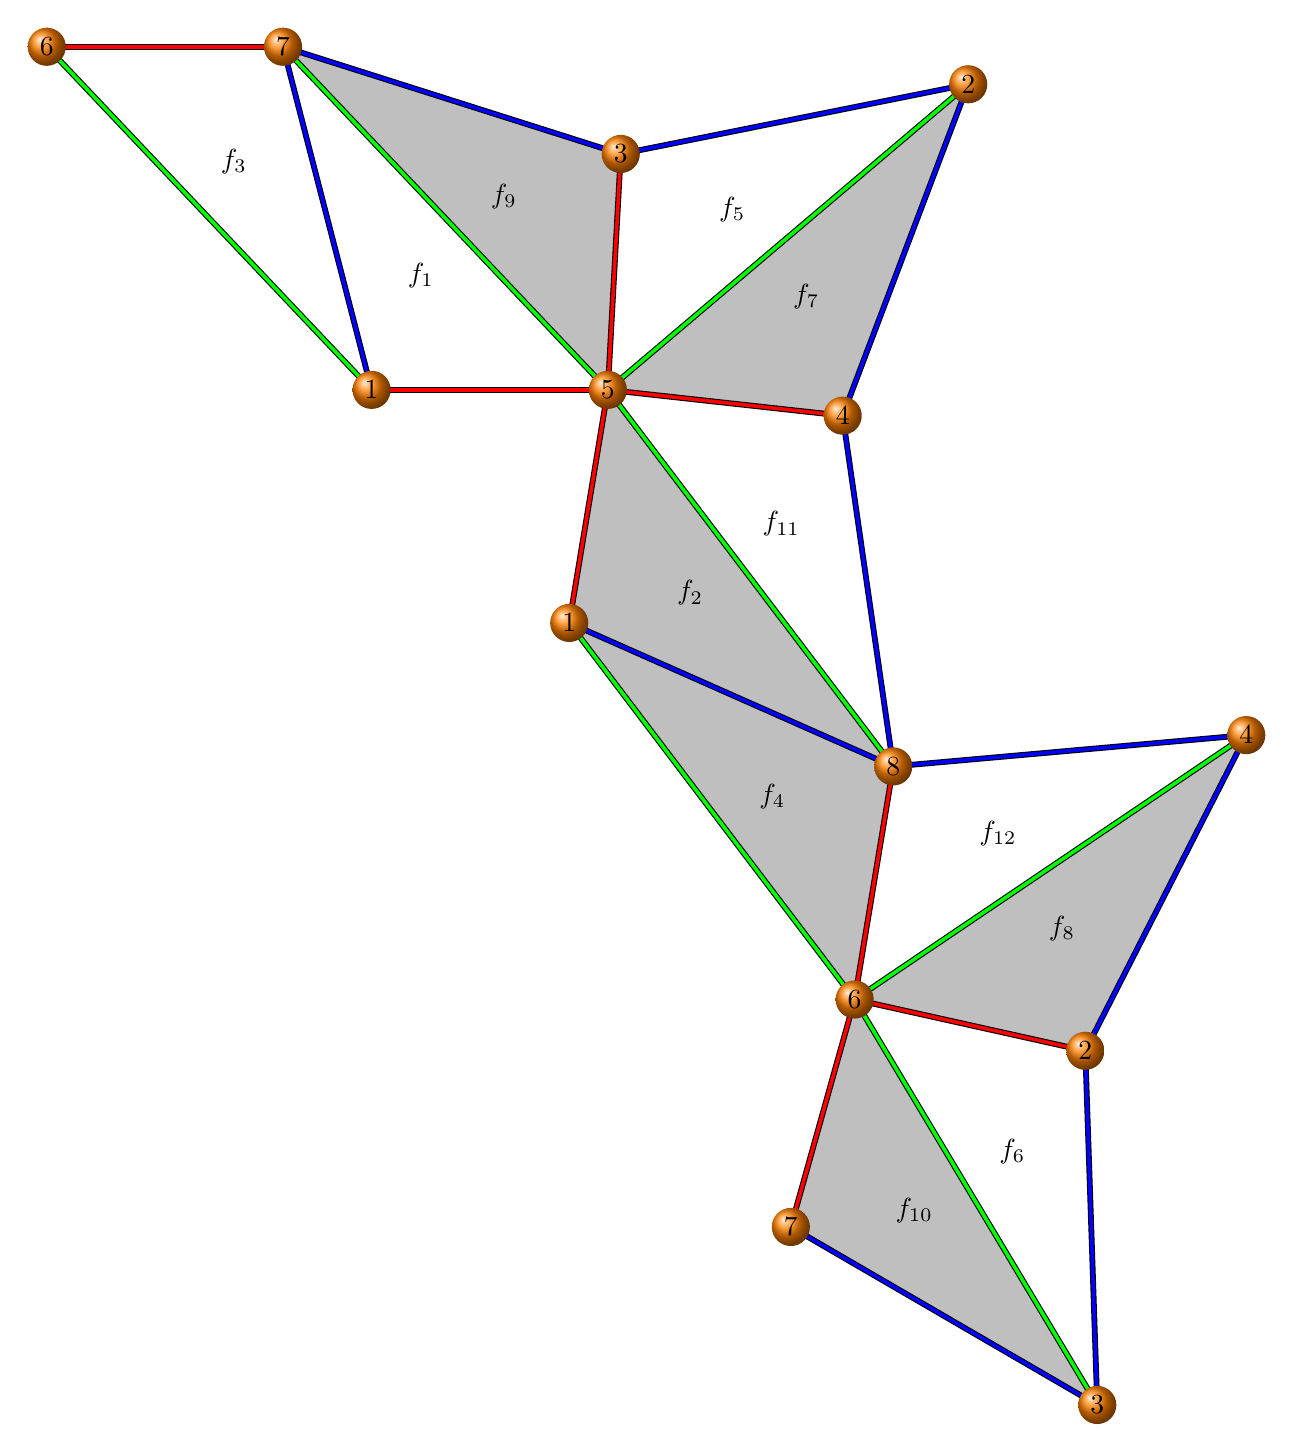
\begin{tikzpicture}[scale=3/2]
\coordinate (V1_1) at (0, 0);
\coordinate (V1_2) at (1.673183441162109, -1.973117061116588);
\coordinate (V2_1) at (5.05078125, 2.587031844536985);
\coordinate (V2_2) at (6.041795790195465, -5.595043502097033);
\coordinate (V3_1) at (2.109375, 1.997007037888199);
\coordinate (V3_2) at (6.1432396620512, -8.593327868340989);
\coordinate (V4_1) at (3.988037109375, -0.2184226447690221);
\coordinate (V4_2) at (7.404570579528809, -2.922433378349563);
\coordinate (V5_1) at (2, 0);
\coordinate (V6_1) at (-2.75, 2.904737509655563);
\coordinate (V6_2) at (4.089504241943359, -5.160811178768384);
\coordinate (V7_1) at (-0.75, 2.904737509655563);
\coordinate (V7_2) at (3.549155795015394, -7.086434079520901);
\coordinate (V8_1) at (4.41632080078125, -3.187694117651796);


\fill[white] (V1_1) -- (V5_1) -- (V7_1) -- cycle;
\node (F1) at (0.4166666666666666, 0.9682458365518543) {$f_{1}$};
\fill[lightgray] (V1_2) -- (V5_1) -- (V8_1) -- cycle;
\node (F2) at (2.69650141398112, -1.720270392922794) {$f_{2}$};
\fill[white] (V1_1) -- (V6_1) -- (V7_1) -- cycle;
\node (F3) at (-1.166666666666667, 1.936491673103709) {$f_{3}$};
\fill[lightgray] (V1_2) -- (V6_2) -- (V8_1) -- cycle;
\node (F4) at (3.393002827962239, -3.440540785845589) {$f_{4}$};
\fill[white] (V2_1) -- (V3_1) -- (V5_1) -- cycle;
\node (F5) at (3.053385416666667, 1.528012960808395) {$f_{5}$};
\fill[white] (V2_2) -- (V3_2) -- (V6_2) -- cycle;
\node (F6) at (5.424846564730008, -6.449727516402135) {$f_{6}$};
\fill[lightgray] (V2_1) -- (V4_1) -- (V5_1) -- cycle;
\node (F7) at (3.679606119791667, 0.7895363999226543) {$f_{7}$};
\fill[lightgray] (V2_2) -- (V4_2) -- (V6_2) -- cycle;
\node (F8) at (5.845290203889211, -4.55942935307166) {$f_{8}$};
\fill[lightgray] (V3_1) -- (V5_1) -- (V7_1) -- cycle;
\node (F9) at (1.119791666666667, 1.633914849181254) {$f_{9}$};
\fill[lightgray] (V3_2) -- (V6_2) -- (V7_2) -- cycle;
\node (F10) at (4.593966566336651, -6.946857708876758) {$f_{10}$};
\fill[white] (V4_1) -- (V5_1) -- (V8_1) -- cycle;
\node (F11) at (3.468119303385417, -1.135372254140273) {$f_{11}$};
\fill[white] (V4_2) -- (V6_2) -- (V8_1) -- cycle;
\node (F12) at (5.303465207417806, -3.756979558256581) {$f_{12}$};


\tikzset{EdgeStyle/.style = {thin, double distance=1.3pt} }

\draw[ EdgeStyle, double=red] (V5_1) -- (V1_1);
\draw[ EdgeStyle, double=red] (V1_2) -- (V5_1);
\draw[ EdgeStyle, double=green] (V1_1) -- (V6_1);
\draw[ EdgeStyle, double=green] (V6_2) -- (V1_2);
\draw[ EdgeStyle, double=blue] (V1_1) -- (V7_1);
\draw[ EdgeStyle, double=blue] (V8_1) -- (V1_2);
\draw[ EdgeStyle, double=blue] (V3_1) -- (V2_1);
\draw[ EdgeStyle, double=blue] (V2_2) -- (V3_2);
\draw[ EdgeStyle, double=blue] (V2_1) -- (V4_1);
\draw[ EdgeStyle, double=blue] (V4_2) -- (V2_2);
\draw[ EdgeStyle, double=green] (V2_1) -- (V5_1);
\draw[ EdgeStyle, double=red] (V2_2) -- (V6_2);
\draw[ EdgeStyle, double=red] (V3_1) -- (V5_1);
\draw[ EdgeStyle, double=green] (V3_2) -- (V6_2);
\draw[ EdgeStyle, double=blue] (V7_1) -- (V3_1);
\draw[ EdgeStyle, double=blue] (V3_2) -- (V7_2);
\draw[ EdgeStyle, double=red] (V4_1) -- (V5_1);
\draw[ EdgeStyle, double=green] (V4_2) -- (V6_2);
\draw[ EdgeStyle, double=blue] (V4_1) -- (V8_1);
\draw[ EdgeStyle, double=blue] (V8_1) -- (V4_2);
\draw[ EdgeStyle, double=green] (V7_1) -- (V5_1);
\draw[ EdgeStyle, double=green] (V8_1) -- (V5_1);
\draw[ EdgeStyle, double=red] (V6_1) -- (V7_1);
\draw[ EdgeStyle, double=red] (V7_2) -- (V6_2);
\draw[ EdgeStyle, double=red] (V8_1) -- (V6_2);



\tikzset{VertexStyle/.style = {
 shape = circle,
 ball color = orange,
 text = black,
 inner sep = 2pt,
 outer sep = 0pt,
 minimum size = 10pt} }

\node[VertexStyle] at (V1_1) {1};
\node[VertexStyle] at (V1_2) {1};
\node[VertexStyle] at (V2_1) {2};
\node[VertexStyle] at (V2_2) {2};
\node[VertexStyle] at (V3_1) {3};
\node[VertexStyle] at (V3_2) {3};
\node[VertexStyle] at (V4_1) {4};
\node[VertexStyle] at (V4_2) {4};
\node[VertexStyle] at (V5_1) {5};
\node[VertexStyle] at (V6_1) {6};
\node[VertexStyle] at (V6_2) {6};
\node[VertexStyle] at (V7_1) {7};
\node[VertexStyle] at (V7_2) {7};
\node[VertexStyle] at (V8_1) {8};

\end{tikzpicture}

\end{document} 
